\documentclass[aspectratio=1610]{beamer}

\usepackage[utf8]{inputenc}
\usepackage{graphicx}
\usepackage{amssymb}
\usepackage{enumitem}
\usepackage[export]{adjustbox}
\usetheme{Frankfurt}
\usefonttheme[onlymath]{serif}

\graphicspath{{./Figures/}}

\definecolor{satinsheengold}{rgb}{0.85, 0.63, 0.21}
\setbeamercolor{structure}{fg=satinsheengold}
\setbeamercolor{title}{fg=black}
\setbeamercolor{title in head/foot}{fg=black, bg=satinsheengold}
\setbeamercolor{author}{fg=black}
\setbeamercolor{frametitle}{fg=black}
\setbeamercolor{author in head/foot}{fg=black, bg=satinsheengold}
\setbeamercolor{institute in head/foot}{bg=satinsheengold}
\setbeamercolor{date in head/foot}{bg=satinsheengold}
\setbeamercolor{navigation symbols}{fg=gray}
\setbeamercolor{block title}{bg=black}
\setbeamercolor{item projected}{fg=black}
\setbeamertemplate{blocks}[rounded][shadow=false]
\setbeamertemplate{enumerate items}[circle]
%\setbeamertemplate{footline}[frame number]
%Adding frame #s
\setbeamertemplate{navigation symbols}{%
    \usebeamerfont{footline}%
    \usebeamercolor[fg]{footline}%
    \hspace{1em}%
    \insertframenumber/\inserttotalframenumber
}

\title{Exploring the Role of Temporal Fine Structure and Envelope in Timbral Coding}
\author{Presented By Andrew Sivaprakasam| BME 511 Fall 2020}

\date{12/07/2020}

\begin{document}

\frame{\titlepage}

\begin{frame}
\frametitle{Music Coding by the Auditory Periphery}

\textit{To appreciate an art, we often must make use of one of our senses. But what happens when our senses are impaired? What kind of signals do we receive from our sensory inputs, and in what fidelity do we receive them? What musical features are most important for us to "lock on" to, and what happens when we can't lock on to them?}\vspace{.5em}

\begin{itemize}[label = $\blacktriangleright$]
\item Musical stimuli are not simple, they are \textbf{often non-periodic and spectrally complicated}
\item If we look \textit{purely} at how we encode components of music, and how important the fidelity we encode those components is, \textbf{we can drive innovative processing algorithms used in hearing aids and cochlear implants to better represent musical sounds}\vspace{1em}

A start would be looking at how \textbf{\textit{\underline{timbre}}} is encoded by the auditory system, and what the signals "look like" before being sent to the brain

\end{itemize}
\end{frame}

\begin{frame}
\frametitle{What is \textit{timbre}?}
\textit{Timbre} is the \textit{\underline{color}} or \textit{\underline{quality}} of a tone perceived by a listener

\begin{columns}
\begin{column}{0.4\textwidth}
\begin{itemize}[label = $\blacktriangleright$]
\item It is a complex psychoacoustic phenomenon that still is not completely understood \vspace{.5em}

\item Timbre is what helps listeners differentiate when the same tone is played by a different instrument \vspace{.5em}

\item Most consider instrumental timbre to be due to the difference in the magnitude of the harmonics of a given tone
%\item  
\end{itemize}
\end{column}
\begin{column}{0.6\textwidth}
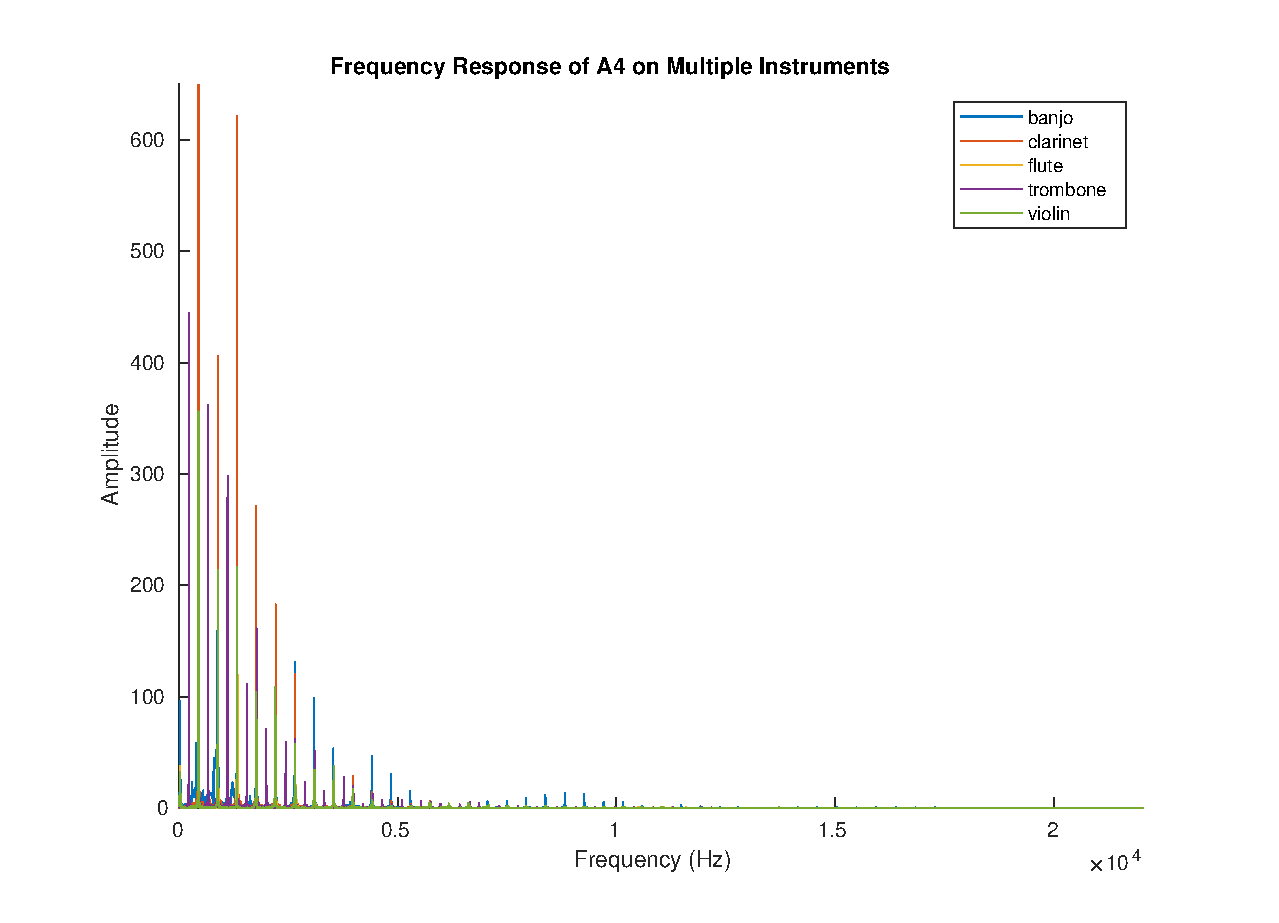
\includegraphics[width = 1.0\textwidth]{fft_all}
\end{column}
\end{columns}

\end{frame}

\begin{frame}
\frametitle{What is \textit{timbre}?}

\begin{columns}
\begin{column}{0.4\textwidth}
\begin{itemize}[label = $\blacktriangleright$]
\item However, envelope is also important\vspace{.5em}
\item In fact, a 2011 study by Heng \textit{et al.} demonstrated that cochlear implant users can differentiate between instruments when 0\% TFS is used in a music-noise chimaera\vspace{.5em}
\item Normal hearing users, however, rely primarily on TFS cues to differentiate instruments
%\item  
\end{itemize}
\end{column}
\begin{column}{0.6\textwidth}
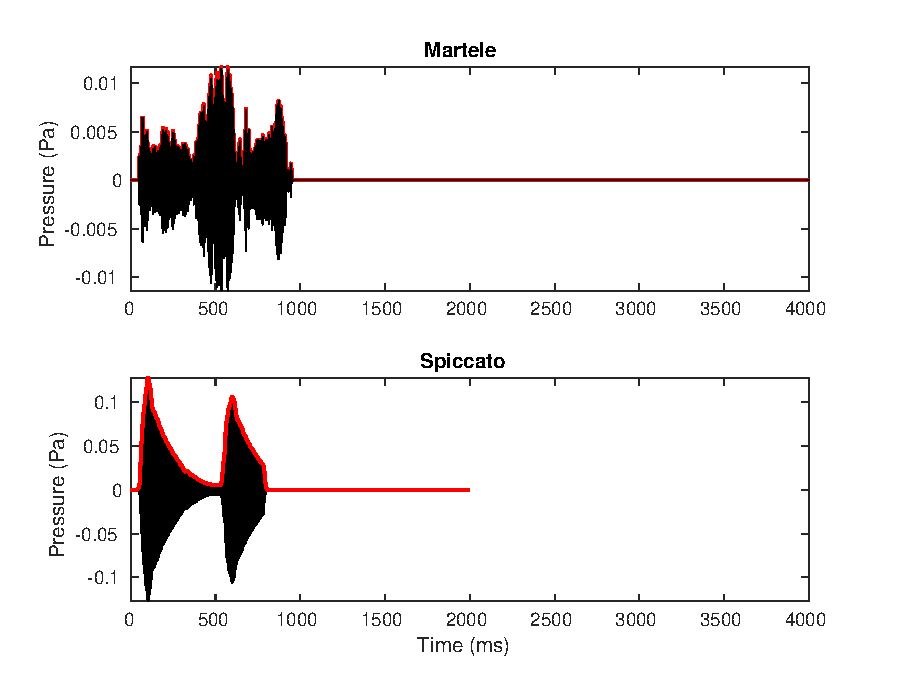
\includegraphics[width = 1.0\textwidth]{martele_spiccato_compare}
\centering
Envelope cues could help us differentiate between different articulations in music, such as \textit{martele} and \textit{spiccato} played by the violin
\end{column}
\end{columns}

\end{frame}

\begin{frame}
\frametitle{Spectrotemporal Analysis}
Spectrograms are an useful tool to visualize differences in instruments. Here are a few of the stimuli I used. The sound samples were collected by the Philharmonia Orchestra in London.\\ 
\vspace{.6em}
\centering
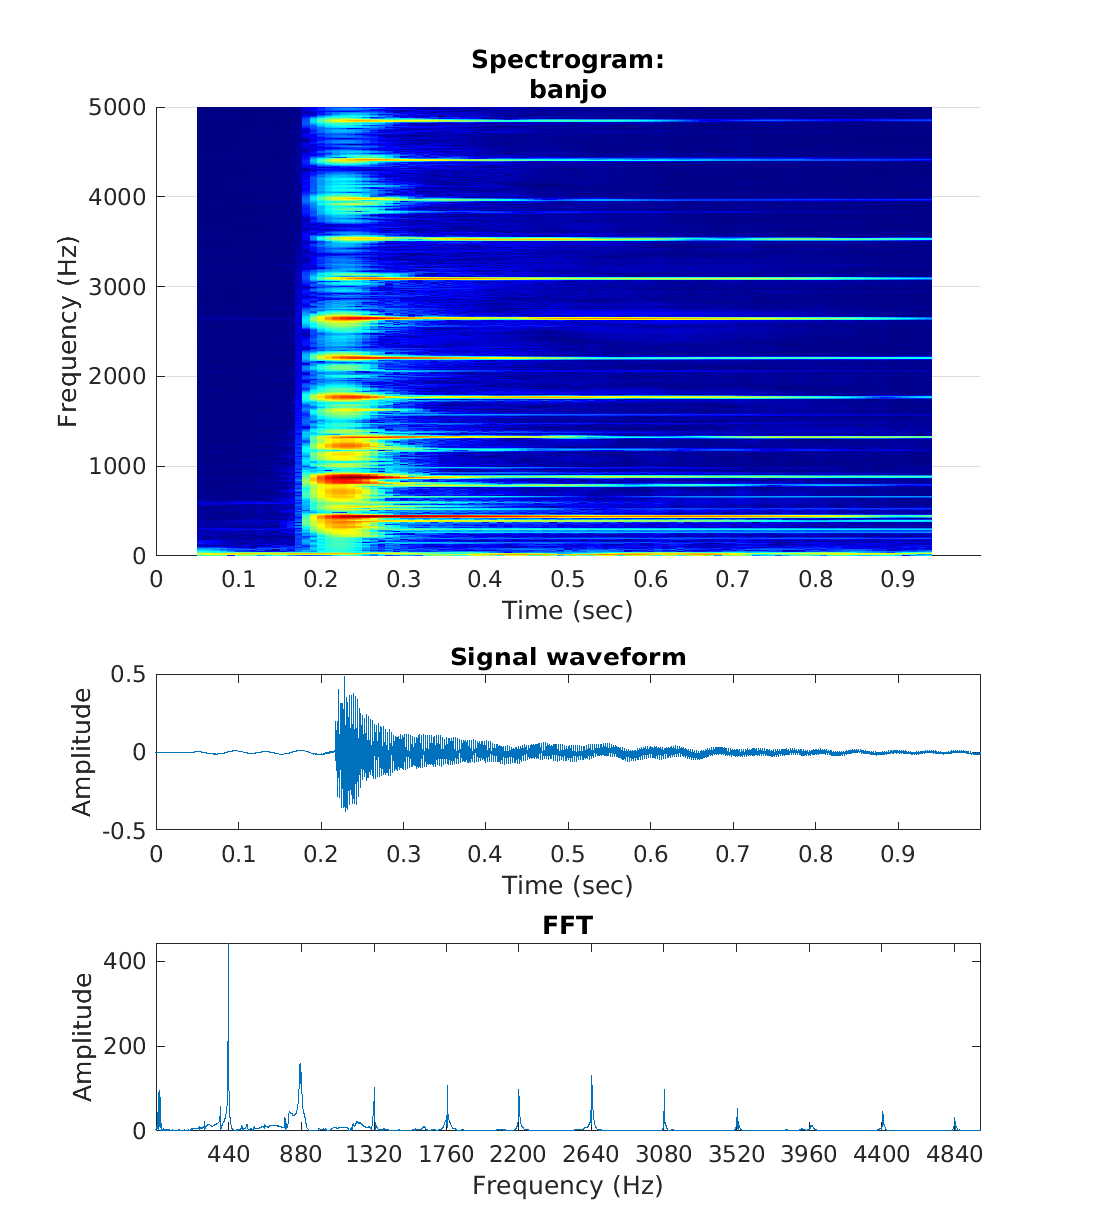
\includegraphics[height = .55\textheight]{spectrogram_banjo}
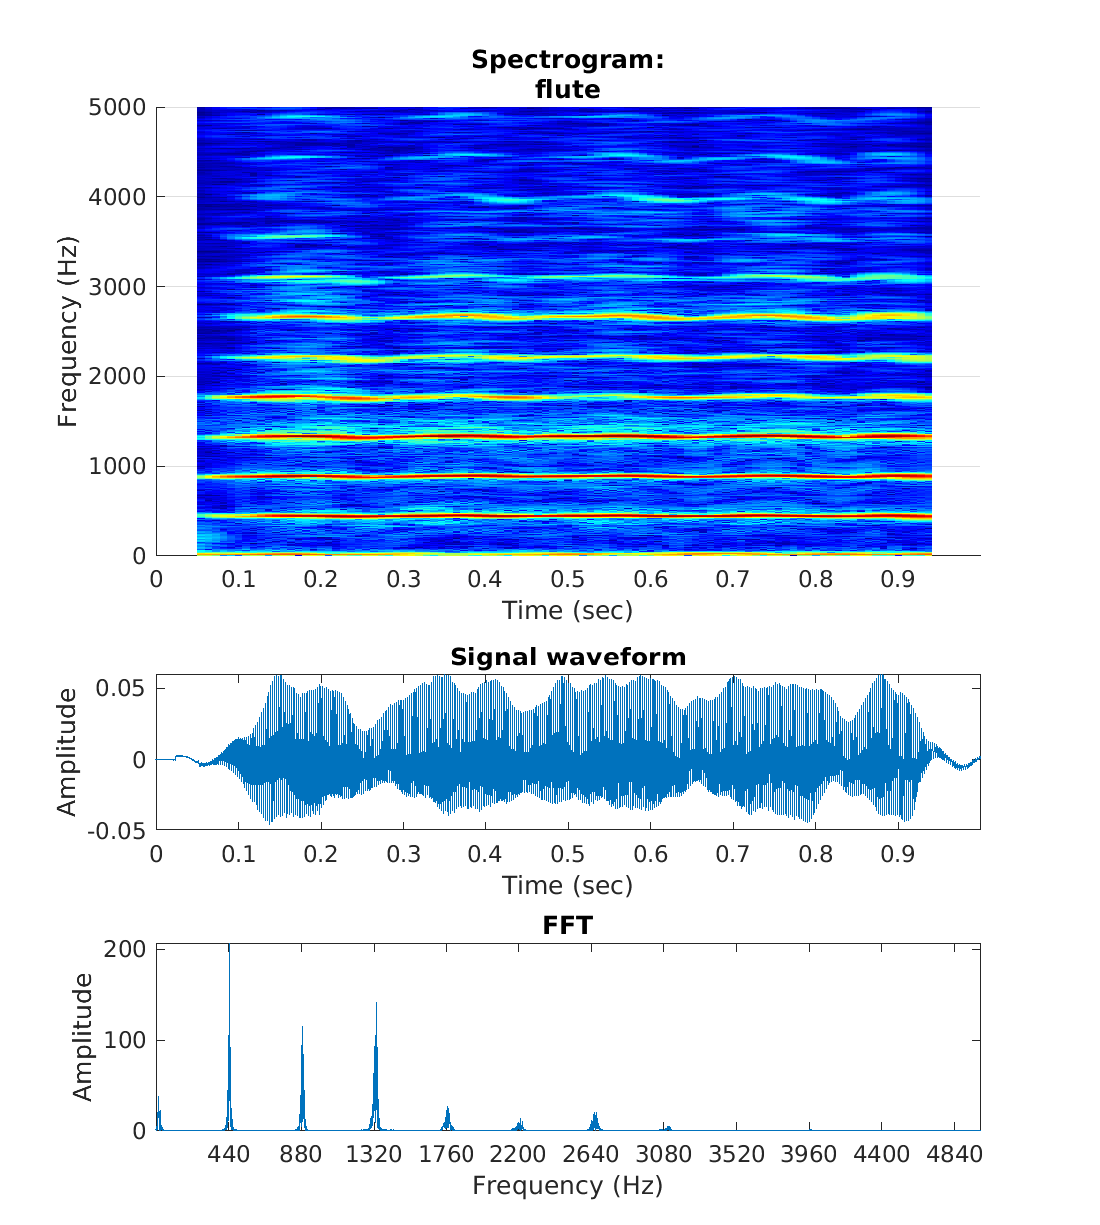
\includegraphics[height = .55\textheight]{spectrogram_flute}
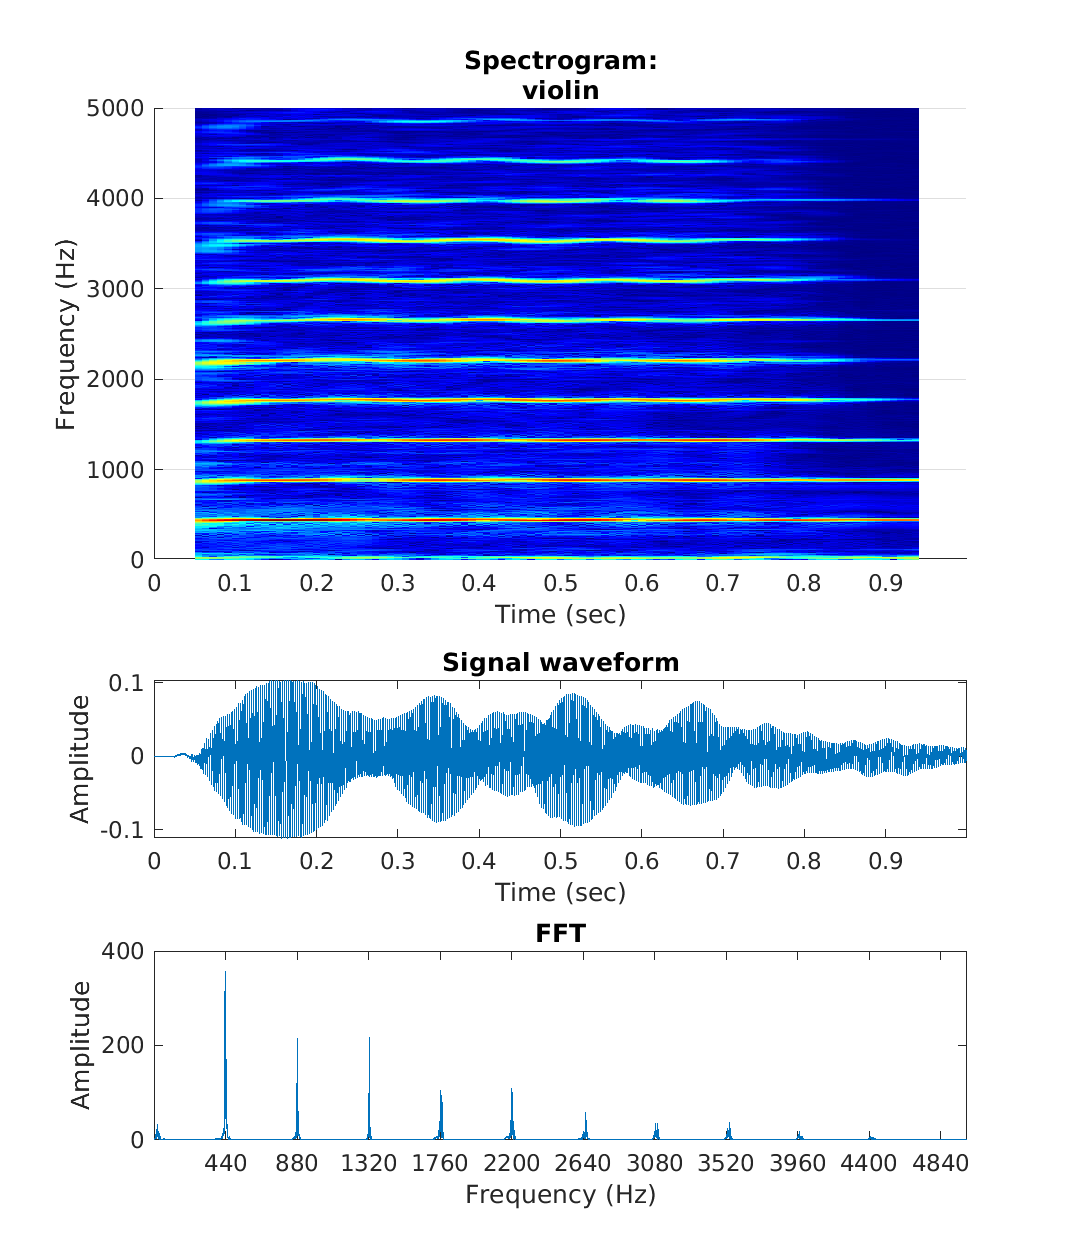
\includegraphics[height = .55\textheight]{spectrogram_violin}
\end{frame}

\begin{frame}
\frametitle{The Idea}

\textbf{\underline{Goal:}} Use a spectrally-specific framework designed to inspect the relevance of TFS and ENV in auditory nerve responses to investigate timbral coding in normal hearing and hearing impaired conditions. \vspace{1em}
\begin{itemize}
\item \textit{\underline{Aim 1:}} \textbf{Instrumental} Timbral Coding:
\begin{itemize}[label = $\blacktriangleright$]
\item Compare timbral coding differences between \textbf{banjo, clarinet, flute, trombone, violin} for a common pitch, \textbf{A4} (440 Hz)
\end{itemize}\vspace{1em}

\item \textit{\underline{Aim 2:}} \textbf{Articulation} Timbral Coding:
\begin{itemize}[label = $\blacktriangleright$]
\item Compare timbral coding differences between two articulations on the violin, \textbf{martel\'{e}} and \textbf{spiccato}
\end{itemize}

\end{itemize}
\end{frame}

\begin{frame}
\frametitle{Modeling Approach}

\begin{itemize}[label = $\blacktriangleright$]
\item Using a model of the auditory nerve developed by Zilany et al. and updated by Bruce et al. in 2018, I was able to quickly collect data. \vspace{.5em}

\item This model can be run in Matlab and also has a variety of customizable parameters.\vspace{.5em}

\item I simulated auditory nerve responses at 4 different Characteristic Frequencies (CF): \\
\begin{center}
125 Hz, $F_0$ (440 Hz), $F_1$ (880 Hz), and $F_9$ (3960 Hz)
\end{center}\vspace{.5em}

\item The Organ of Corti in the cochlea can be thought of as a filterbank with filters centered around a given CF (the further down the cochlea you go, the lower the CF) 
\end{itemize}

\end{frame}

\begin{frame}
\frametitle{Modeling Approach}
This model also allowed adjustment of Outer Hair Cell and Inner Hair Cell parameters based on an audiogram. I chose hearing loss threshold shifts roughly based on data reported by Tufts et al. in a 2005 study of musical interval consonance:\vspace{1em} 

\centering
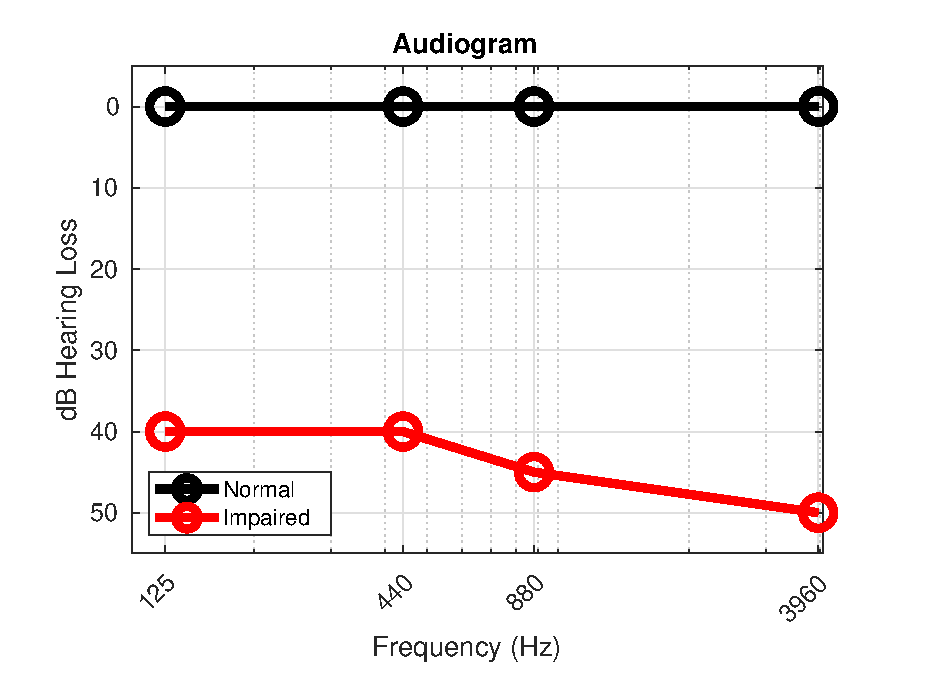
\includegraphics[width = .6\textwidth]{audiogram} 

\end{frame}

\begin{frame}
\frametitle{Modeling Approach}


\centering

\includegraphics[width = 1\textwidth]{bruce} \vspace{1em} 
A schematic of the original Zilany Model. Sound stimulus goes in, spike train comes out. 

\end{frame}

\begin{frame}
\frametitle{General Methods Overview}


\centering

\includegraphics[height = .77\textheight]{methods_pics} \vspace{1em} 


\end{frame}


\end{document}